%!TEX root=../thesis.tex
\chapter{Teorema de Poincaré-Bendixson} \label{cap:poincarebendixson}

\section{Conjuntos límite y nociones básicas}

Ya hemos encontrado diversos tipos de órbitas en sistemas planos: órbitas constantes de la forma $\gamma_{\bar{x}} = \{\bar{x}\}$ en el caso de equilibrios $\bar{x}$, órbitas periódicas y órbitas que se ``alejan'' hacia infinito.
De hecho la situación es más rica, existen órbitas límites a las cuales se acercan arbitrariamente órbitas cercanas (por ejemplo, vistas en el diagrama de fase \ref{fig:vanderpol}). Esto no es inusual y se trata de hecho de una situación típica en el plano.

Hemos estudiado también lo que sucede con soluciones que empiezan ``cerca'' de puntos de equilibrio y hemos visto que algunas tienden a dichos puntos de equilibrio cuando $t \to \infty$ (o más precisamente $t \to \beta_{x_0}$) cuando los puntos son asintóticamente estables, se alejan (cuando los equilibrios son inestables) o corresponden a órbitas periódicas en el caso de equilibrios que son centros.

Formalizamos esto con el concepto de $\alpha$-límite y $\omega$-límite.

\begin{definition}Sean $x \in \R^2$, $\phi(t,x)$ el flujo a través de $x$ e $I_x = (\alpha_x, \beta_x)$ el intervalo (posiblemente infinito) de definición de la solución a través de $x$ garantizada por el teorema de existencia.

\begin{enumerate}[(a)]
	\item $y\in \R^2$ se dice un \emph{punto $\alpha$-límite de $x$} si existe una sucesión de tiempos $\{ t_k \}_k \subseteq I_x$ tal que $t_k \to \alpha_x$ y $\phi(t_k, x) \to y$ cuando $k \to \infty$.
	\item $z\in \R^2$ se dice un \emph{punto $\omega$-límite de $x$} si existe una sucesión de tiempos $\{ t_k \}_k \subseteq I_x$ tal que $t_k \to \beta_x$ y $\phi(t_k, x) \to z$ cuando $k \to \infty$.
\end{enumerate}

\end{definition}

Al conjunto de todos los puntos $\alpha$-límite de $x$ se le llama \emph{conjunto $\alpha$-límite de $x$} y se denota por $\alpha(x)$. Análogamente, $\omega(x)$ denota al conjunto de todos los puntos $\omega$-límite de $x$, llamado \emph{conjunto $\omega$-límite de $x$}.

Debido a que si $x$ es un punto de la órbita $\gamma$ entonces $\phi(t,x) \in \gamma$ para todo $t$ por definición de órbita, utilizamos indistintamente la notación $\omega(x)$ u $\omega(\gamma)$ para denotar el conjunto límite de dicha órbita.

Ahora, la discusión precedente implica que las órbitas $\gamma$ cercanas a puntos de equilibrio asintóticamente estables $\bar{x}$ tienen conjunto límite $\omega(\gamma) = \{\bar{x}\}$. Si $\bar{x}$ no es asintóticamente estable podría suceder que $\gamma$ sea no acotada (y se aleja a infinito), $\gamma$ es periódica y en este caso coincide con su conjunto límite $\omega(\gamma)$ o bien, $\gamma$ se acerca arbitrariamente a otra órbita $\tau$ que debe ser periódica.

Este tipo de comportamientos límite de las órbitas se han evidenciado hasta ahora en los ejemplos estudiados pero resulta que, de hecho, el comportamiento de las órbitas en el plano es siempre uno de este tipo, como asegura el Teorema de Poincaré-Bendixson que probaremos en la sección siguiente.

Sin pérdida de generalidad trabajaremos únicamente con las semiórbitas positivas $\gamma^+$ (obviando $t < 0$) y solo con conjuntos $\omega$-límite. Resultados idénticos aplican para conjuntos $\alpha$-límite y semiórbitas negativas $\gamma^-$ generalmente con tan solo ``reversar'' el tiempo con una transformación $t \mapsto -t$.

Introducimos ahora la noción de conjunto invariante.

\begin{definition} \label{def:conjuntoinvariante}
Un conjunto $A \subseteq \R^2$ es \emph{invariante} respecto al sistema $\dot{x} = f(x)$ si $\phi(t,x) \in A$ para todo $x \in A$ y $t \in I_x$.
\end{definition}

Equivalentemente, $A$ es un conjunto invariante si es una unión de órbitas.

% TODO: ejemplos

\begin{lemma} \label{lem:orbitaslimite}
Sea $\gamma^+(x)$ la semiórbita positiva de un punto $x \in \R^2$. Si $\gamma^+(x)$ es acotada entonces:

	\begin{enumerate}[(a)]
		\item $\omega(x)$ es no vacío, compacto y conexo.
		\item $d(\phi(t,x), \omega(x)) \to 0$ cuando $t \to \infty$.
		\item $\omega(x)$ es un conjunto invariante del sistema plano. En particular, si $y \in \omega(x)$ entonces $\gamma^+(y) \subseteq \omega(x)$.
	\end{enumerate}
\end{lemma}

\begin{proof}
\begin{enumerate}[(a)]
	\item Sea $x \in \R^2$. Probaremos que: (i) $\omega(x)$ es no vacío, (ii) acotado (iii) cerrado (iv) conexo.

	(i) Construimos la sucesión $(x_i)$ definida por $ x_i:= \phi(i, x), i \in \N$. Como $\{x_i\}_i \subseteq \gamma^+(x)$ y $\gamma^+(x)$ está acotada por hipótesis entonces la sucesión también está acotada. Por lo tanto, existe una subsucesión convergente, digamos, a $p$. Claramente, $p \in \omega(x)$ por definición así que $\omega(x) \neq \emptyset$.

	(ii) Si $\omega(x)$ fuera no acotado entonces existirían sucesiones $(t_i)$ tales que $\phi(t_i, x)$ es no acotada cuando $i \to \infty$ (o de lo contrario $\omega(x)$ sería acotado), pero como $\phi(t_i, x) \in \gamma^+(x)$ para todo $i$ entonces esto implica que la semiórbita positiva $\gamma^+(x)$ es no acotada, una contradicción.

	(iii) Que $\omega(x)$ es cerrado se sigue de un típico argumento de puntos límites tomando una sucesión $y_i \in \omega(x)$ que converge a $p$ y considerando las respectivas sucesiones $\phi(t_k^{(i)}, x)$ tales que $\phi(t_k^{(i)}, x) \to y_i$ cuando $i \to \infty$. Se puede construir entonces una sucesión de algunos de tales $t_k^{(i)}$ tal que $\phi(t_k^{(i)}, x) \to p$, probando así que $p \in \omega(x)$.

	(iv) Para ver que $\omega(x)$ es conexo supongamos que $\omega(x) = A \cup B$ con $A,B$ subconjuntos no vacíos, acotados, cerrados y disjuntos de $\R^n$.
	Como $A$ y $B$ son cerrados y disjuntos entonces $d(A,B) = \delta > 0$. Ya que $A$ y $B$ están formados por puntos $\omega$-límite entonces existen sucesiones de tiempos $(t_i^A)$ y $(t_i^B)$ tales que

$$ d(A, \phi(t_i^A, x)) < \frac{\delta}{2}, \text{ y } d(B, \phi(t_i^B, x)) < \frac{\delta}{2}$$

lo que implica que

$$ d(A, \phi(t_i^B, x)) > \frac{\delta}{2}. $$

Por continuidad de la función distancia $d$ y $\phi$ se sigue que existe una sucesión $(\tau_j)$ de tiempos tal que

$$ d(A, \phi(\tau_j, x)) = \frac{\delta}{2}. $$

Como $(\phi(\tau_j, x))_j$ es una sucesión acotada debe tener una subsucesión convergente. Podemos suponer que $(\phi(\tau_j, x))_j$ misma converge a $z$ cuando $j \to \infty$ , pero entonces $z \in \omega(x)$ por definición y $z$ satisface que $d(z,A) = \delta/2$ de manera que $z \notin A$ y también

$$ d(z,B) \geq d(A,B) - d(z,A) = \delta/2$$

así que $z \notin B$. Esto es una contradicción pues $\omega(x) = A \cup B$.

\item Veamos ahora que $d(\phi(t,x), \omega(x)) \to 0$ cuando $t \to \infty$. Supongamos que no, entonces existe $\delta > 0$ y una sucesión $(t_i)$ tal que 

$$ d(\phi(t_i, x), \omega(x)) \geq \delta > 0.$$

Como la sucesión $(\phi(t_i, x))$ está en un conjunto acotado admite una subsucesión convergente. Sin pérdida de generalidad podemos suponer que $(\phi(t_i, x))$ misma es convergente, digamos, a $p$ cuando $t \to \infty$. Claramente $p \in \omega(x)$ pero entonces por la desigualdad anterior y la continuidad de la distancia $d$ y $\phi$ debe tenerse que

$$ d(p, \omega(x)) > 0,$$

una contradicción pues $p \in \omega(x)$.

\item Finalmente veamos que $\omega(x)$ es invariante. Consideramos únicamente invariancia positiva: es decir, debemos ver que dado $u \in \omega(x)$ entonces todo $v = \phi(t, u)$ está en $\omega(x)$ para $t > 0$. La invariancia negativa (es decir, para $t < 0$) se prueba análogamente.

Por definición existe una sucesión $t_i$ tal que

$$ x_i = \phi(t_i, x) \to u$$

cuando $i \to \infty$. Consideramos la sucesión

$$ y_i := \phi(t, x_i) = \phi(t, \phi(t_i, x)).$$

Como $\phi$ es continua en ambos argumentos entonces

$$ y_i \to \phi(t, u) = v$$

cuando $i \to \infty$.

Pero también $ \phi(t, \phi(t_i, x)) = \phi(t + t_i, x) $ por la propiedad de semigrupo del espacio de tiempos de un sistema dinámico. Esto implica que si hacemos $\tau_i := t + t_i$ entonces

$$ \phi(\tau_i, x) \to v$$

cuando $i \to \infty$ lo que significa que $v \in \omega(x)$ por definición de punto de $\omega$-límite.
\end{enumerate}
\end{proof}

\begin{corollary}[Transitividad] Sean $x,y,z \in \R^2$. Si $z \in \omega(y)$ y $y \in \omega(x)$ entonces $z \in \omega(x)$.
\end{corollary}

\section{Teorema de Poincaré-Bendixson}

Como hemos dicho, el Teorema de Poincaré-Bendixson permite clasificar completamente el comportamiento límite de la órbita de cualquier punto $x \in \R^2$ en un sistema dinámico plano.

La idea es que la órbita $\gamma(x)$ de un punto $x$ puede ser no acotada (en cuyo caso, la órbita se ``aleja'' a infinito) o bien es acotada y sucede una de dos posibilidades: el conjunto límite $\omega(\gamma)$ consta de un número finito de puntos críticos y $\gamma$ tiende a uno de ellos cuando $t \to \infty$ o $\omega(\gamma)$ es una órbita periódica.

Por supuesto si $\gamma$ ya es una órbita periódica entonces $\gamma = \omega(\gamma)$. En caso contrario, nos encontramos precisamente con lo que se conoce como órbita ``límite'' que es necesariamente periódica.

Que el sistema dinámico sea plano es de vital importancia: este tipo de comportamiento es exclusivo de los sistemas dinámicos planos y la razón de esto yace en el Teorema de la Curva de Jordan (ver \cite{fleming,spivak}) que aplica únicamente sobre $\R^2$.

En el camino a la prueba del teorema de Poincaré-Bendixson, utilizaremos la noción de segmento transversal.

\begin{definition}Un segmento cerrado rectilíneo $L$ es \emph{transversal} a $\dot{x} = f(x)$ si el vector $f$ no se anula en $L$ (no hay equilibrios en $L$) y es no tangente a $L$ en todo punto de $L$.
\end{definition}

\begin{figure}[h] \centering
    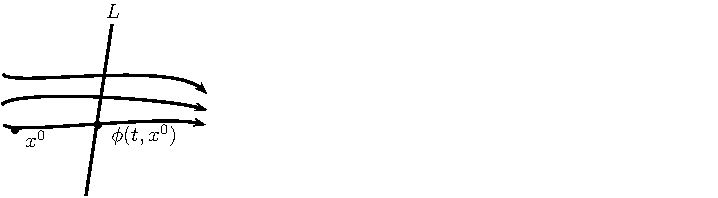
\includegraphics[scale=1.1]{figures/transversal.pdf}
\end{figure}

Es claro que en vecindad de un punto regular $x$ (es decir, $f(x) \neq 0$) siempre es posible construir un segmento transversal $L$ por la continuidad de $f$.

El resultado clave que involucra conjuntos $\omega$-límite y transversales es el siguiente.

\begin{lemma} \label{lem:transversalexistencias}

Sea $p \in \omega(x)$ y $L$ un segmento transversal a través de $p$. Para todo $\epsilon > 0$ existe una vecindad $V_\epsilon(p)$ tal que toda órbita que pasa a través de un punto interior de $V_\epsilon(p)$ para $t = 0$ cruza a $L$ para algún tiempo $s$, $|s| < \epsilon$. 
\end{lemma}
\begin{proof}
Sea $a \in \R^2$ un vector ortogonal al segmento $L$, de manera que para todo punto $q \in L$ se tiene

$$ \langle a, q-p \rangle = 0.$$

Definamos la función $g(x,s)$ por

$$ g(x,s) := \langle a, \phi(s, x) - p \rangle.$$

Claramente $g$ es suave y está definida cerca de $(p,0)$ y $g(p,0) = 0$. Además, $g_s(p,0) = \langle a, f(p) \rangle \neq 0$ pues $L$ es un segmento transversal a $f$.

Bajo estas hipótesis el teorema de la función implícita (ver \cite{spivak,fleming}) garantiza la existencia de una función $\tau: x \mapsto \tau(x)$ suave tal que $\tau(p) = 0$ definida en una vecindad $V_\epsilon(p)$ y tal que en dicha vecindad se satisface

$$ g(x, \tau(x)) = 0. $$

O lo que es lo mismo, si $y$ es cualquier punto en $V_\epsilon(p)$ entonces con el tiempo $s = \tau(y)$ se obtiene que $\phi(s, y)$ está en $L$.

\end{proof}

\begin{proposition}Dado $x \in \R^2$ y un segmento transversal $L$ la intersección $\omega(x) \cap L$ contiene a lo más un punto.
\end{proposition}

\begin{proof}
Supongamos que $\omega(x) \cap L$ es no vacío y sea $q \in \omega(x) \cap L$. Por definición de $\omega$-límite existe una sucesión $t_k$ de tiempos tal que $\phi(t_k, x) \to q$ cuando $k \to \infty$. Por el lema anterior para cada uno de estos $t_k$ existe un $s_k$ con $|s_k| > |t_k|$ tal que $x_k = \phi(t_k + s_k, x)$ está en $L$.

Consideramos dos casos:

(i) Si $(x_k)_k$ es una sucesión constante entonces la órbita de $x$ es periódica y $\omega(x) = \gamma(x)$, así que el $\omega$-límite de $x$ solo puede intersectar a $L$ en el valor constante $(x_k)_k$ y por lo tanto $\omega(x) \cap L = \{q\}$.

(ii) Si $(x_k)_k$ no es constante consideremos dos puntos sucesivos $x_k$ y $x_{k+1}$ donde $\omega(x)$ intersecta a $L$, como en la figura \ref{fig:transversalintersections}. Como $L$ es transversal a $f$ entonces a lo largo de $L$ el campo vectorial $f$ debe apuntar en una dirección diferente a la de $L$ (esto pues $L$ no es tangencial a $f$ en ningún punto) y además debe hacerlo siempre en esa misma dirección ya que de lo contrario, por continuidad de $f$, sería posible encontrar $z \in L$ tal que $f(z) = 0$, lo que contradice la definición de $L$.

Ahora, el segmento de órbita entre $x_k$ y $x_{k+1}$ junto con el segmento rectilíneo entre esos dos puntos forma una curva cerrada $C$. Como consecuencia del Teorema de la Curva de Jordan, esta curva $C$ divide al plano $\R^2$ en dos componentes conexas: una acotada y otra no acotada.

Dependiendo de la ubicación de $x_k$ y $x_{k+1}$ sobre $L$ y debido a la dirección de $f$ sobre dicha transversal las únicas posibilidades son que la semiórbita positiva $\gamma^+(x_k)$ esté siempre contenida en la componente acotada o siempre contenida en la no acotada, como ilustra la figura \ref{fig:transversalintersections}. En cualquier caso, debe tenerse que la siguiente intersección $x_{k+2}$ se encuentre por fuera del segmento entre $x_k$ y $x_{k+1}$, lo que obliga a que los puntos $x_k$, $x_{k+1}$ y $x_{k+2}$ estén ordenados en la transversal $L$.

En estas condiciones $(x_k)_k$ es una sucesión monótona sobre un segmento rectilíneo y puede tener, por tanto, a lo más un punto de acumulación en $L$, como se quería probar. Esto es, $\omega(x) \cap L = \{q\}$.

\end{proof}

\begin{figure}[h] \centering
    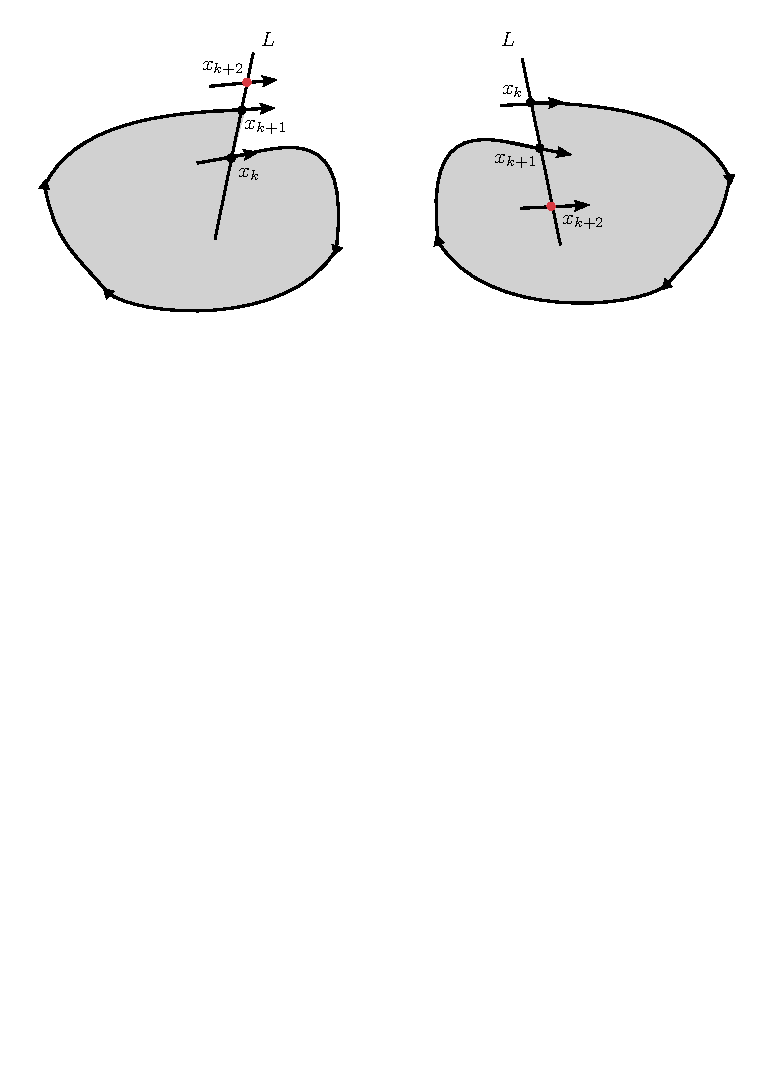
\includegraphics[scale=1.15]{figures/transversalintersections.pdf}
	\caption{Intersecciones con la transversal $L$.}
	\label{fig:transversalintersections}
\end{figure}

\begin{theorem}[Poincaré-Bendixson] \label{teo:poincarebendixson} Sea $f:\R^2 \to \R^2$ una función de clase $C^1$. Para el sistema plano $\dot{x} = f(x)$, si la semiórbita positiva $\gamma^+(x)$ de algún punto $x$ está acotada y $\omega(x)$ no contiene puntos críticos entonces $\omega(x)$ es una órbita periódica (órbita límite).
\end{theorem}

\begin{proof}
Del lema \ref{lem:orbitaslimite} se sigue que $\omega(x)$ es no vacío, compacto y conexo. Sea $p \in \omega(x)$, se sigue por transitividad que $\omega(p) \subseteq \omega(x)$. Ahora sea $q \in \omega(p)$. Por hipótesis, $q$ no es un punto crítico así que existe un segmento transversal a $f$, $L$, a través de $q$.  Como $q \in \omega(p)$ existe una sucesión de tiempos $(t_k)$ tal que $\phi(t_k, p) \to q$ cuando $k \to \infty$.

Por el lema \ref{lem:transversalexistencias} podemos suponer de una vez que $\phi(t_k, p) \in L$ para todo $k \in \N$. Ahora, como $p \in \omega(x)$ entonces $\gamma^+(p) \subseteq \omega(x)$ por lema \ref{lem:orbitaslimite}. Esto es lo mismo que $\phi(t_k, p) \in \omega(x)$ para todo $k \in \N$.

Ahora, como $\phi(t_k, p) \in \omega(x) \cap L$ entonces por la proposición precedente,

$$ \phi(t_k, p) = q  \hspace{0.5in} \forall k \in \N.$$

Esto implica que $\gamma(p)$ es una órbita periódica y ya sabemos que $\gamma(p) \subseteq \omega(x)$. Resta probar la otra contención.
Si $\omega(x) \backslash \gamma(p) \neq \emptyset$ entonces como $\omega(x)$ es conexo se sigue que cada vecindad de $\gamma(p)$ contiene puntos de $\omega(x)$ que no están en $\gamma(p)$.
Ahora, estas vecindades pueden tomarse suficientemente pequeñas para que no contengan puntos críticos, de manera que existan segmentos transversales a $f$, $L'$ conteniendo uno de estos puntos que están en $\omega(x)$ y un punto de $\gamma(p)$. Por lo tanto $\omega(x) \cap L'$ contiene al menos dos puntos pues $\gamma(p) \subseteq \omega(x)$ pero esto contradice la proposición anterior.
Debe tenerse entonces que $\omega(x) \backslash \gamma(p) = \emptyset$ así que $\omega(x) = \gamma(p)$, es decir, el $\omega$-límite de $x$ es una órbita periódica.

\end{proof}

Estamos en condiciones de probar que las únicas posibilidades para los conjuntos $\omega$-límite de una órbita son las consideradas al inicio del capítulo como ejemplos típicos.

\begin{corollary} \label{teo:poincarebendixson2} Sea $f: \R^2 \to \R^2$ de clase $C^1$. Para el sistema plano $\dot{x} = f(x)$ si la semiórbita positiva $\gamma^+$ de un punto $x$ está contenida en un conjunto compacto $K$ de $\R^2$ donde hay a lo más un número finito de puntos críticos, entonces se cumple alguno de estos:

	\begin{enumerate}[(a)]
		\item $\omega(\gamma^+)$ consiste de un solo punto crítico  y $\gamma^+$ se aproxima a este cuando $t \to \infty$;
		\item $\omega(\gamma^+)$ es una órbita periódica;
		\item $\omega(\gamma^+)$ consiste de un número finito de puntos críticos y órbitas que tienden a estos puntos cuando $t \to \pm \infty$.
	\end{enumerate}
\end{corollary}

\begin{proof}
\begin{enumerate}[(a)]
	\item Como $\omega(\gamma^+) \subseteq \overline{\gamma^+} \subseteq K$ entonces $\omega(\gamma^+)$ contiene a lo más un número finito de puntos críticos. Si contiene alguno entonces debe ser necesariamente un solo punto crítico pues $\omega(x)$ es conexo (no puede ser unión de varios puntos críticos). Claramente $\gamma^+$ tiende a este punto crítico cuando $t \to \infty$.
	\item Supongamos ahora que $\omega(\gamma^+)$ no contiene puntos críticos. Por teorema \ref{teo:poincarebendixson} $\omega(\gamma^+)$ debe ser una órbita periódica.
	\item Suponemos ahora que $\omega(\gamma^+)$ contiene un número finito de puntos críticos pero ninguna órbita periódica. Sea $\gamma_0$ cualquier órbita en $\omega(\gamma^+)$. Por el caso (a) debe tenerse que $\alpha(\gamma_0)$ o $\omega(\gamma_0)$ consisten de un único punto crítico y por lo tanto $\gamma_0$ tiende a uno de estos cuando $t \to \pm \infty$.
\end{enumerate}
\end{proof}

\begin{example} \label{ex:poincarebendixson}
Consideremos el sistema en coordenadas polares dado por

\begin{equation} \label{eq:expoincarebendixson}
	\begin{array}{lll}
		\dot{r} & = & r(1-r) \\
		\dot{\theta} & = & 1.
	\end{array}
\end{equation}

El diagrama de fase de este sistema es el mostrado en la figura \ref{fig:expoincarebendixson}.

Es fácil verificar que $\omega(x) = S^1$ para todo $x$, donde $S^1$ es el círculo de radio 1 con centro en el origen. Con esto sabemos, de antemano, de la existencia de un ciclo límite en este sistema (a saber, $S^1$).

Las ecuaciones \ref{eq:expoincarebendixson} permiten este análisis por su naturaleza sencilla, pero podemos corroborar este hecho a través del teorema \ref{teo:poincarebendixson} utilizando únicamente el acotamiento.

\begin{figure}[!htb] \centering
	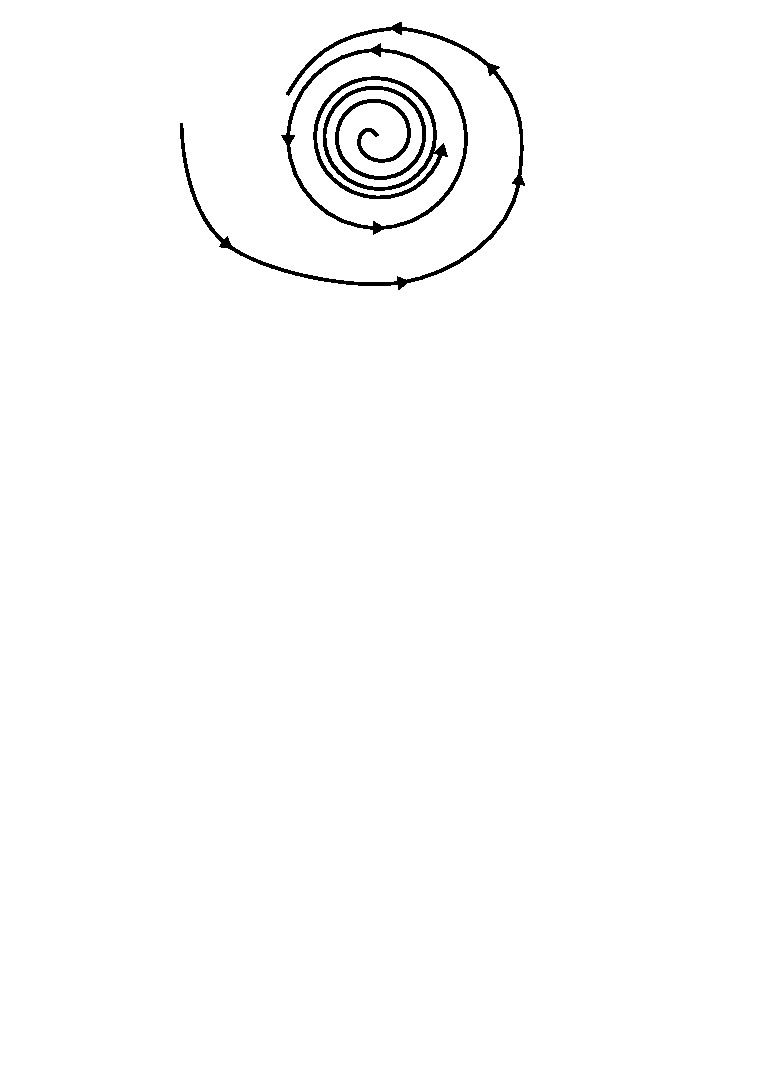
\includegraphics[scale=1.1]{figures/expoincarebendixson.pdf}
	\caption{Diagrama de fase de la ecuación \ref{eq:expoincarebendixson}.}
	\label{fig:expoincarebendixson}
\end{figure}

Para ello consideramos el anillo
$$ A := \left\{ x \in \R^2 : \frac{1}{2} < ||x|| < 2 \right\} $$

que corresponde a la región polar $\frac{1}{2} < r < 2$ y $\theta \in [0,2\pi]$.

Para $r = 1/2$ se tiene $\dot{r} = 1/4 > 0$ y para $r = 2$ se tiene $\dot{r} = -2 < 0$ lo que implica que toda órbita que entre a $A$ debe permanecer en $A$ para $t \geq 0$.
Por ejemplo, si tal órbita ingresara a $A$ desde ``adentro'' (cruzando $r = 1/2$) y se acercara a la frontera $r = 2$ entonces la condición $\dot{r} < 0$ implicaría que $r$ debe disminuir sobre dicha órbita, es decir, la órbita debe ``introducirse'' de nuevo en $A$. La condición $\dot{r} > 0$ en $r = 1/2$ obliga también a que la órbita no pase al disco interior $r < 1/2$ y por tanto permanezca siempre dentro del anillo $A$.

Esta situación es ilustrada en la figura \ref{fig:expoincarebendixson2}.

En particular, cualquier semiórbita positiva $\gamma^+(x)$ de un punto $x \in A$ está contenida en $A$, que es acotado, y por tanto es acotada. Como además es claro que el origen es el único punto crítico del sistema se sigue del teorema de Poincaré-Bendixson que $\omega(x)$ es una órbita periódica para todo $x \in A$. Esto es, un ciclo límite.

\begin{figure}[!ht] \centering
	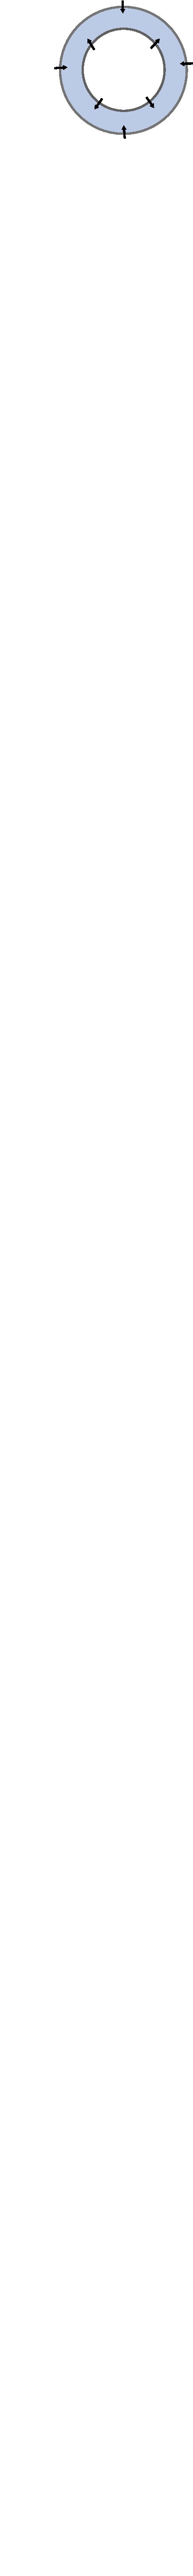
\includegraphics[scale=1.0]{figures/expoincarebendixson2.pdf}
	\caption{Comportamiento cualitativo cerca de la frontera de $A$.}
	\label{fig:expoincarebendixson2}
\end{figure}

\end{example}
	